\documentclass[a4paper, 12pt]{article}

\usepackage{graphicx}
\usepackage{caption}
\usepackage[section]{placeins}
\usepackage{fixltx2e}
\usepackage[page]{appendix}

\usepackage{amsmath}
\usepackage{cleveref}

%for code(MATLAB in particular)
\usepackage{listings}
\usepackage{color} %red, green, blue, yellow, cyan, magenta, black, white
\definecolor{mygreen}{RGB}{28,172,0} % color values Red, Green, Blue
\definecolor{mylilas}{RGB}{170,55,241}

% Default fixed font does not support bold face
\DeclareFixedFont{\ttb}{T1}{txtt}{bx}{n}{12} % for bold
\DeclareFixedFont{\ttm}{T1}{txtt}{m}{n}{12}  % for normal

% Custom colors
\usepackage{color}
\definecolor{deepblue}{rgb}{0,0,0.5}
\definecolor{deepred}{rgb}{0.6,0,0}
\definecolor{deepgreen}{rgb}{0,0.5,0}


\newcommand\pythonstyle{\lstset{
language=Python,
basicstyle=\ttm,
otherkeywords={self},             % Add keywords here
keywordstyle=\ttb\color{deepblue},
emph={MyClass,__init__},          % Custom highlighting
emphstyle=\ttb\color{deepred},    % Custom highlighting style
stringstyle=\color{deepgreen},
frame=tb,                         % Any extra options here
showstringspaces=false            % 
}}

\lstnewenvironment{python}[1][]
{
\pythonstyle
\lstset{#1}
}
{}

\newcommand\pythonexternal[2][]{{
\pythonstyle
\lstinputlisting[#1]{#2}}}


\lstset{
    language=Matlab,%
    %basicstyle=\color{red},
    breaklines=true,%
    morekeywords={matlab2tikz},
    keywordstyle=\color{blue},%
    morekeywords=[2]{1}, keywordstyle=[2]{\color{black}},
    identifierstyle=\color{black},%
    stringstyle=\color{mylilas},
    commentstyle=\color{mygreen},%
    showstringspaces=false,%without this there will be a symbol in the places where there is a space
    numbers=left,%
    numberstyle={\tiny \color{black}},% size of the numbers
    numbersep=9pt, % this defines how far the numbers are from the text
    emph=[1]{for,end,break},emphstyle=[1]\color{red}, %some words to emphasise
    %emph=[2]{word1,word2}, emphstyle=[2]{style},
}


\graphicspath{{./pictures/}}

\title{ECEN321 - Lab 1}
\author{Joshua Benfell - 300433229}

\begin{document}
	\maketitle
    
    \section{Introduction}
        This report investigates three types of distribution; Normal, T and Chi$^2$. The purpose of this investigation is to firstly, further understand these distributions and secondly to see how accurately the experimental data matches with the theory.
    \section{Theory}
        \subsection{Normal Distribution} \label{sec:normalTheory}
            For this distribution 1000 normally distributed variables were generated using the \textbf{randn()} function from the Python library, numpy. This was done around a mean of 2.5 with a variance of 16; standard deviation of 4. This generated a list of normally distributed variables.
            $$
                \mu + randn(N) * \sigma
            $$
            After this list was created, the mean, variance and standard devitation were obtained from the sample so that they could be compared with the input variables. For visual comparison to a normal distribution, the sample was plotted as a histogram in 30 bins. To allow comparison with the probability density function (PDF) of the normal distribution the histogram had to be scaled to a probability mass function (PMF). This was done by first scaling the bin heights by the total number of sample points, and then scaling by the width of the bins.

            \begin{python}
H,X = np.histogram(nums, bins = 30)
dx = X[1] - X[0]
histProbabilities = H / (N * dx)
            \end{python}

            \begin{equation}\label{eq:pdf}
                p(x; \mu, \sigma^2) = \frac{1}{\sqrt{2 \pi \sigma^2}} \exp{\left(-\frac{(x-\mu)^2}{2\sigma^2}\right)}
            \end{equation}

            Using \cref{eq:pdf}, the theoretical and experimental PDFs were calculated and plotted along side the scaled histogram.
            \par
            The other aspect of this distribution to compare is the cumulative distribution function (CDF) of the experimental data from the histogram and for both the population mean and variance and those of the sample. The theoretical CDFs where calculated with \cref{eq:cdfNormal}, where erf is the error function from the scipy library and the empirical CDF of the histogram was done using the cumulative summation function (cumsum) in the numpy library.

            \begin{equation}\label{eq:cdfNormal}
                \phi(x) = \frac{1}{2} \left( 1 + erf \left( \frac{x-\mu}{\sigma \sqrt{2}}\right) \right)  \cite{mathworksErf}
            \end{equation}
        \subsection{Student t Distribution} \label{sec:stTheory}
            To ivestigate the t distribution, a matrix of size $5_M \times 10000_N$ was filled with normally distributed samples with the same mean and variance as that described in \cref{sec:normalTheory}. From this sample each column of the matrix was operated on making a t-value for that column using \cref{eq:tval}. This equation uses the standard deviation of the entire matrix, the true mean and the mean of the column.
            \begin{equation}\label{eq:tval}
                \frac{\left(\mu_{column} - \mu_{true}\right)}{\sigma_{sample}} \times \sqrt{M}
            \end{equation}
            The t-values were then plotted on a histogram using the same method described in \cref{sec:normalTheory}. Plotted alongside this was theoretical PDF (tPDF) for degrees of freedom $\nu =M - 1 = 4$. On a second plot, the sorted data was plot against the rank alongside the theoretical CDF (tCDF).
        \subsection{Chi$^{2}$ Density}
            This density was investigates by first, generating a matrix in the same way as the one in \cref{sec:stTheory}. This time, chi squared values were made by taking the sample variance for each column and dividing it by the $\frac{5-1}{\sigma^2}$. This was plotted alongside the tPDF for 4 (M-1) and 5 (M) degrees of freedom using the chi2.pdf method in the scipy library. This was repeated on a second plot but instead of the sample variance where it's the difference from the sample mean, the difference from the true mean was used.
    \section{Results and Discussion}
        \subsection{Normal Distribution} \label{sec:normalExp}
            \begin{figure}[!h]
                \centering
                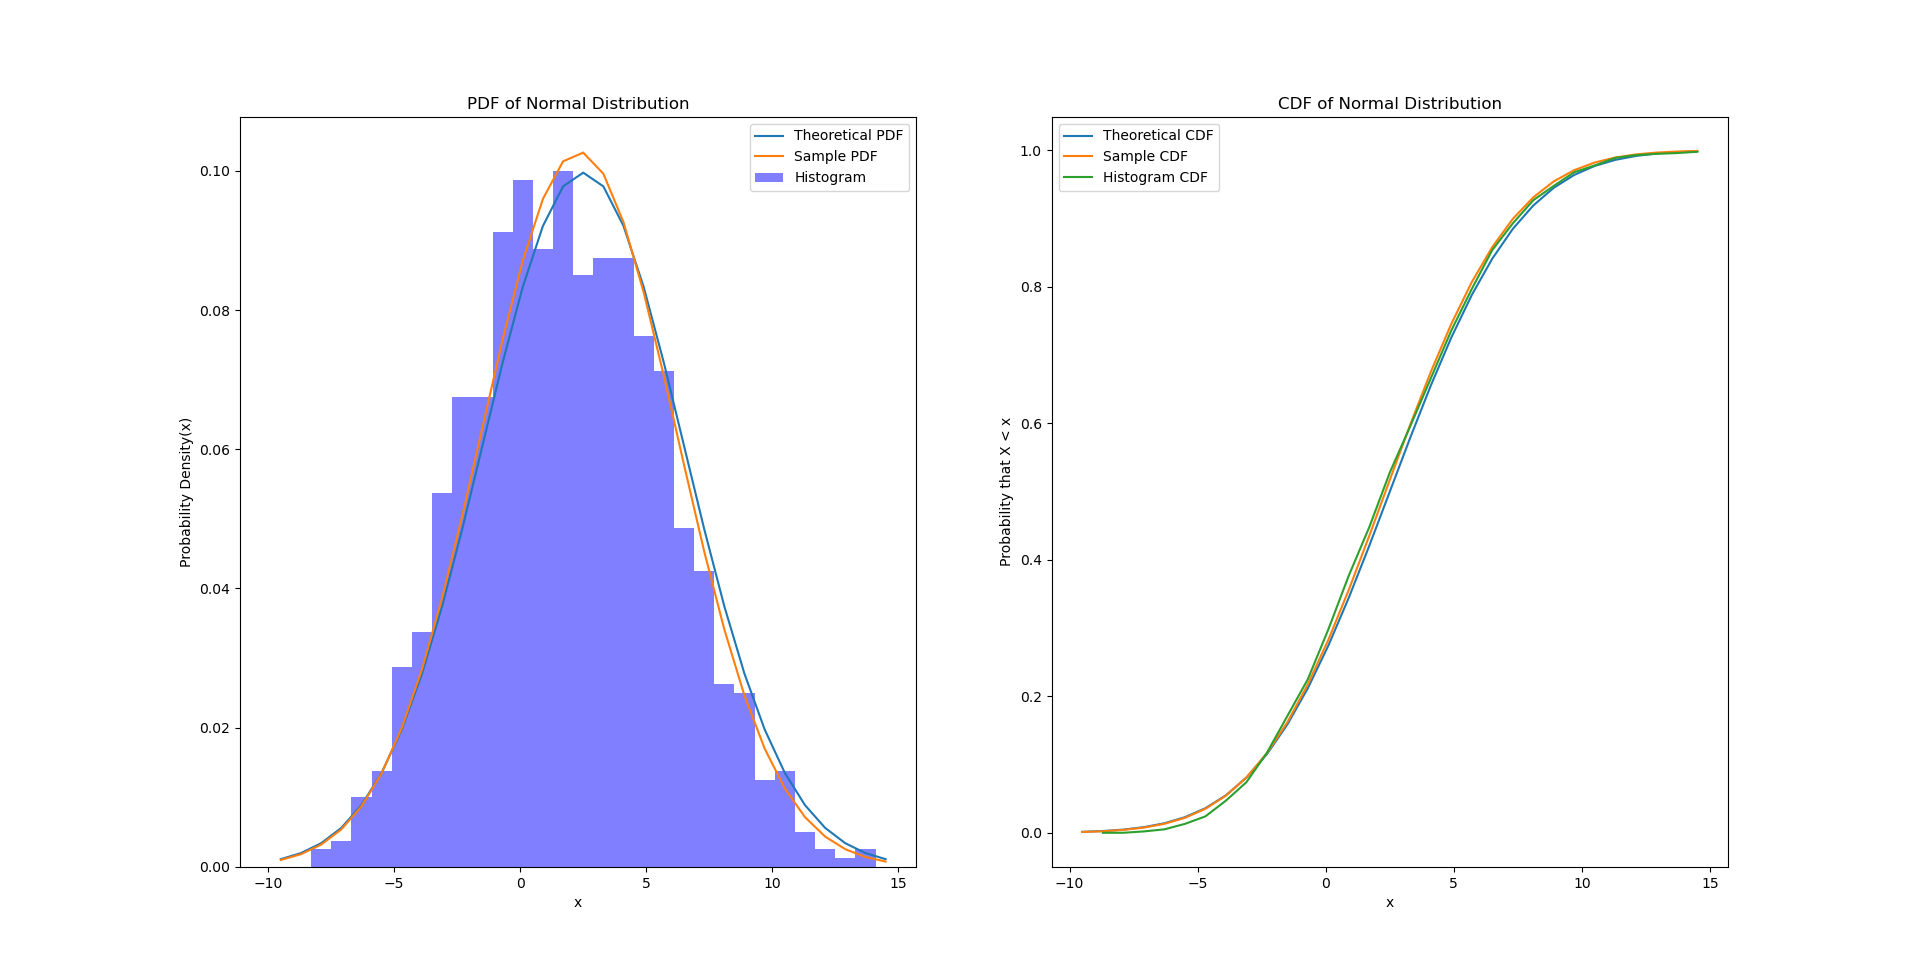
\includegraphics[width=0.95\textwidth]{normal.png}
                \caption{PDFs and CDFs of the normal distribution with true mean of 2.5}
                \label{fig:normal}
            \end{figure}

            The resulting plots from the python script written for this distribution can be seen in \cref{fig:normal}. The following values relate to this sample set:
            \begin{itemize}
                \item $\mu$: 2.332364394985525
                \item $\sigma^2$: 15.086094766162631
                \item $\sigma$: 3.8840822295830235
            \end{itemize}
            From the above list we can see that the values of the sample have minor differences from the true values that the set was generated from. This is reflected in the plot as it can be seen that the general shape of the pmf is similar to the theoretical pdf. For this particular sample it is better reflected in the experimental pdf, both are left leaning but it is less exagerrated in the pdf.
            \par
            Both the theoretical and experimental CDFs are very close to each other that any difference is minor. The CDF from the pmf has got clearer differences in it. This is reflected in the pmf as it can be seen that many more data points happen early on in this sample which causes the cdf to be above the tCDF in the second plot. 
            \par
            Because both of these plots have results that closely resemble the theory it can be concluded that the theory behind the normal distribution matches the experimental results.
        \subsection{Student t Distribution} \label{sec:tExp}
            \begin{figure}[!h]
                \centering
                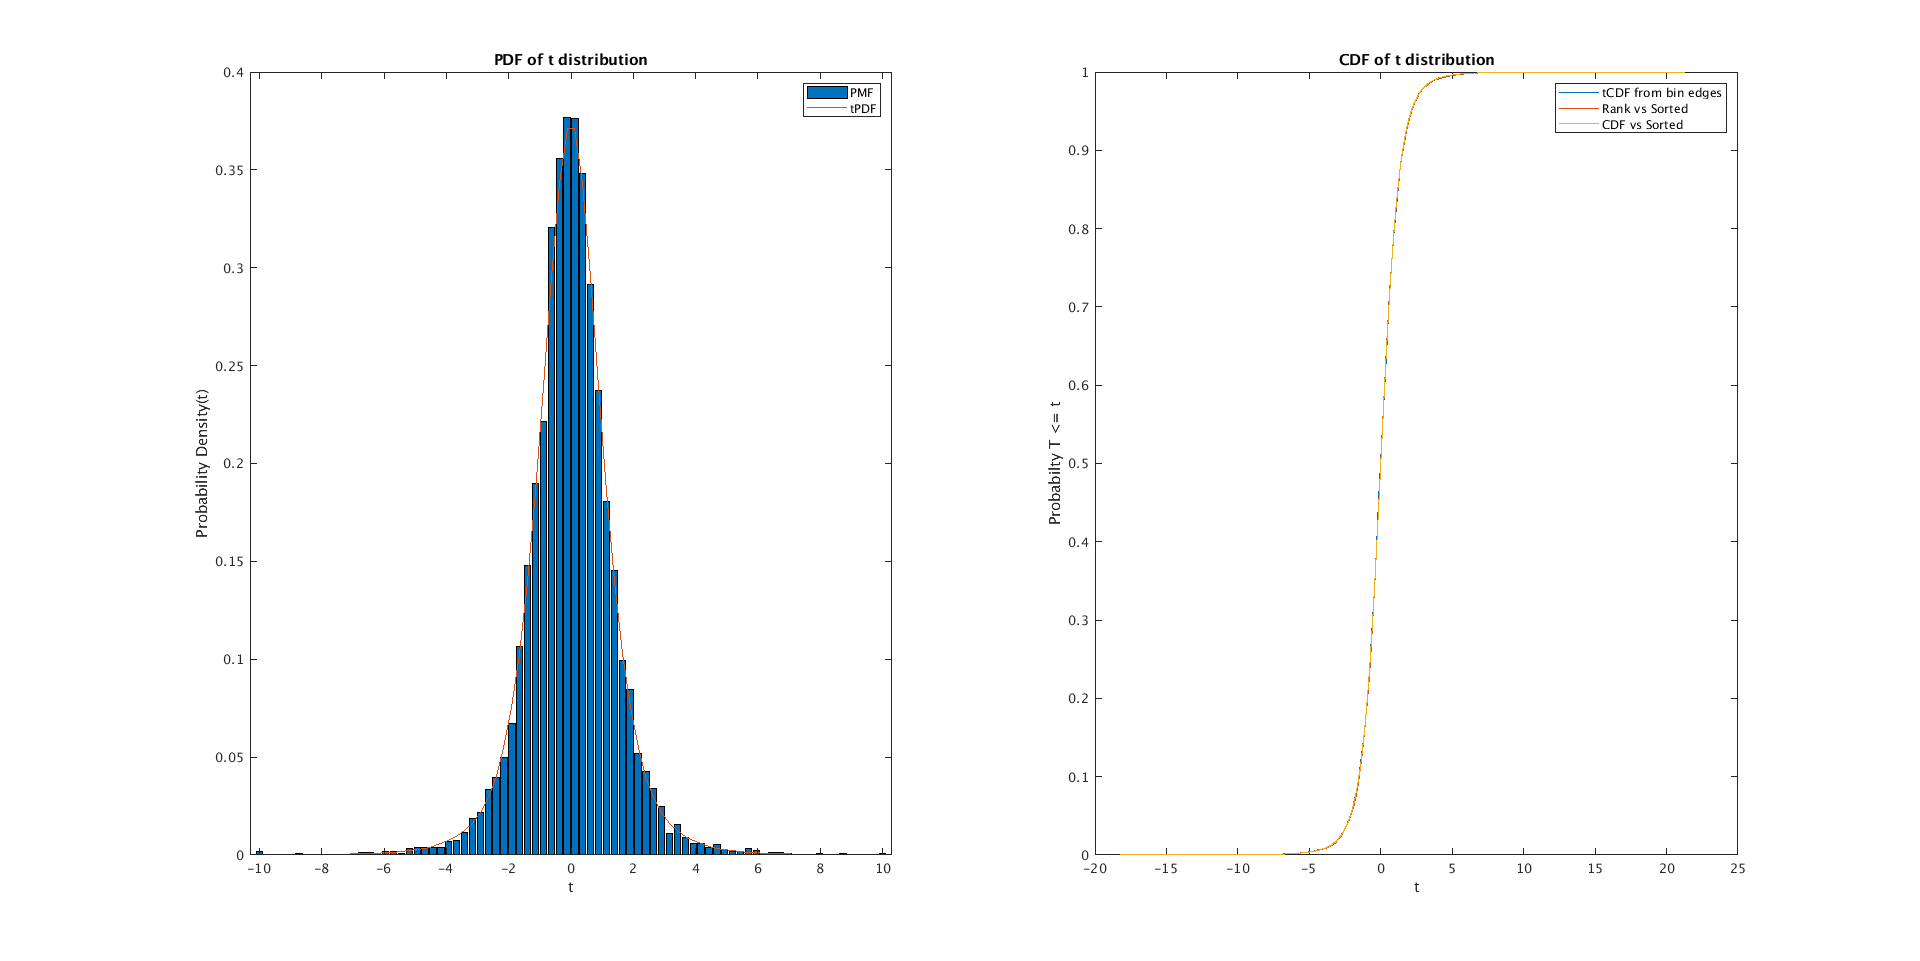
\includegraphics[width=0.95\textwidth]{t.png}
                \caption{PDFs and CDFs of the t distribution with true mean of 2.5}
                \label{fig:t}
            \end{figure}
            \begin{figure}[!h]
                \centering
                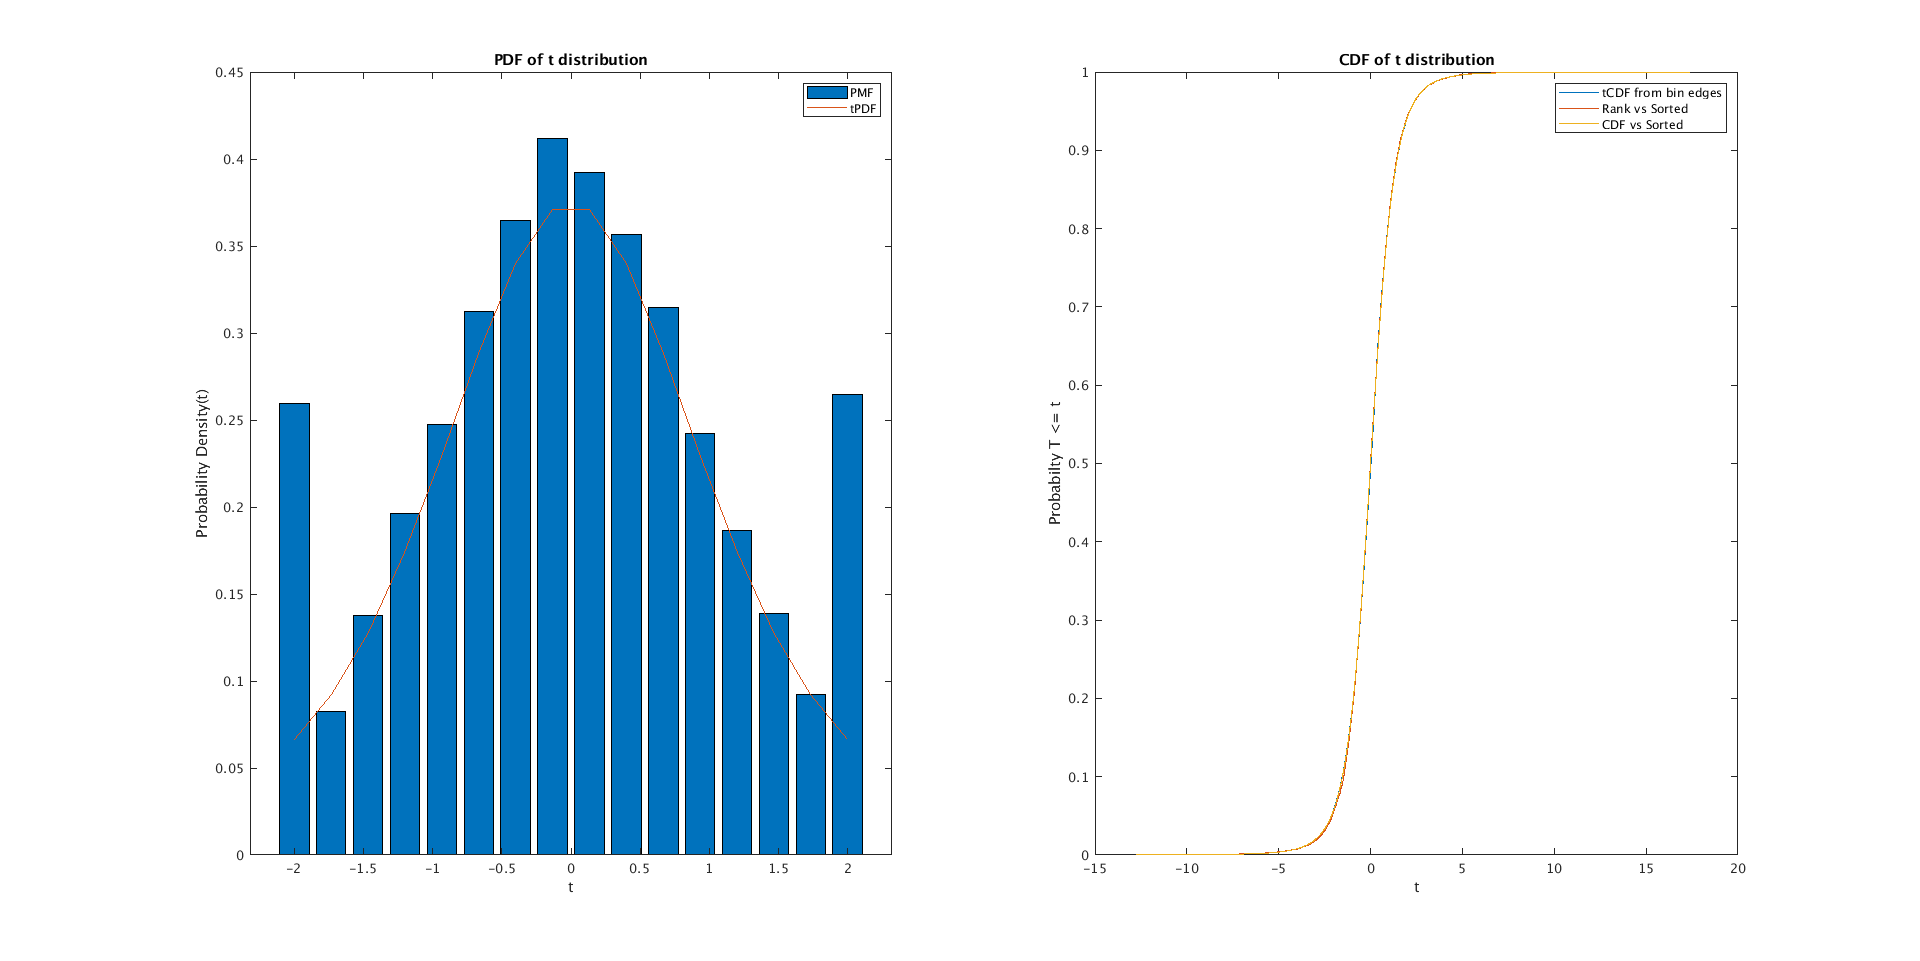
\includegraphics[width=0.95\textwidth]{tSmallRange.png}
                \caption{PDFs and CDFs of the t distribution with true mean of 2.5 over a small range}
                \label{fig:tSmallRange}
            \end{figure}
            The resulting plots for this experiment can be seen in \cref{fig:t}. The experiment probability density lines up along the edges almost exactly with the theoretical pdf. This holds true for the cdf and tcdf as there is very little difference between the two lines. The tcdf was compared against two other plots, the cdf made from the pmf (histogram) and from plotting the sorted data against the rank. Both ended up being very close to the theoretical line. This indicates that the t distribution holds true for normally distributed random variables.
            \par
            There was some issue with generating this plot. If the range of the x axis that the histogram was generated on was too small (between $\pm$2 in \cref{fig:tSmallRange}) it would shoot up on the sides due to the long tails. This is remedied by specifying a larger range.
        \subsection{Chi$^{2}$ Density} \label{sec:chi2Exp}
            \begin{figure}
                \centering
                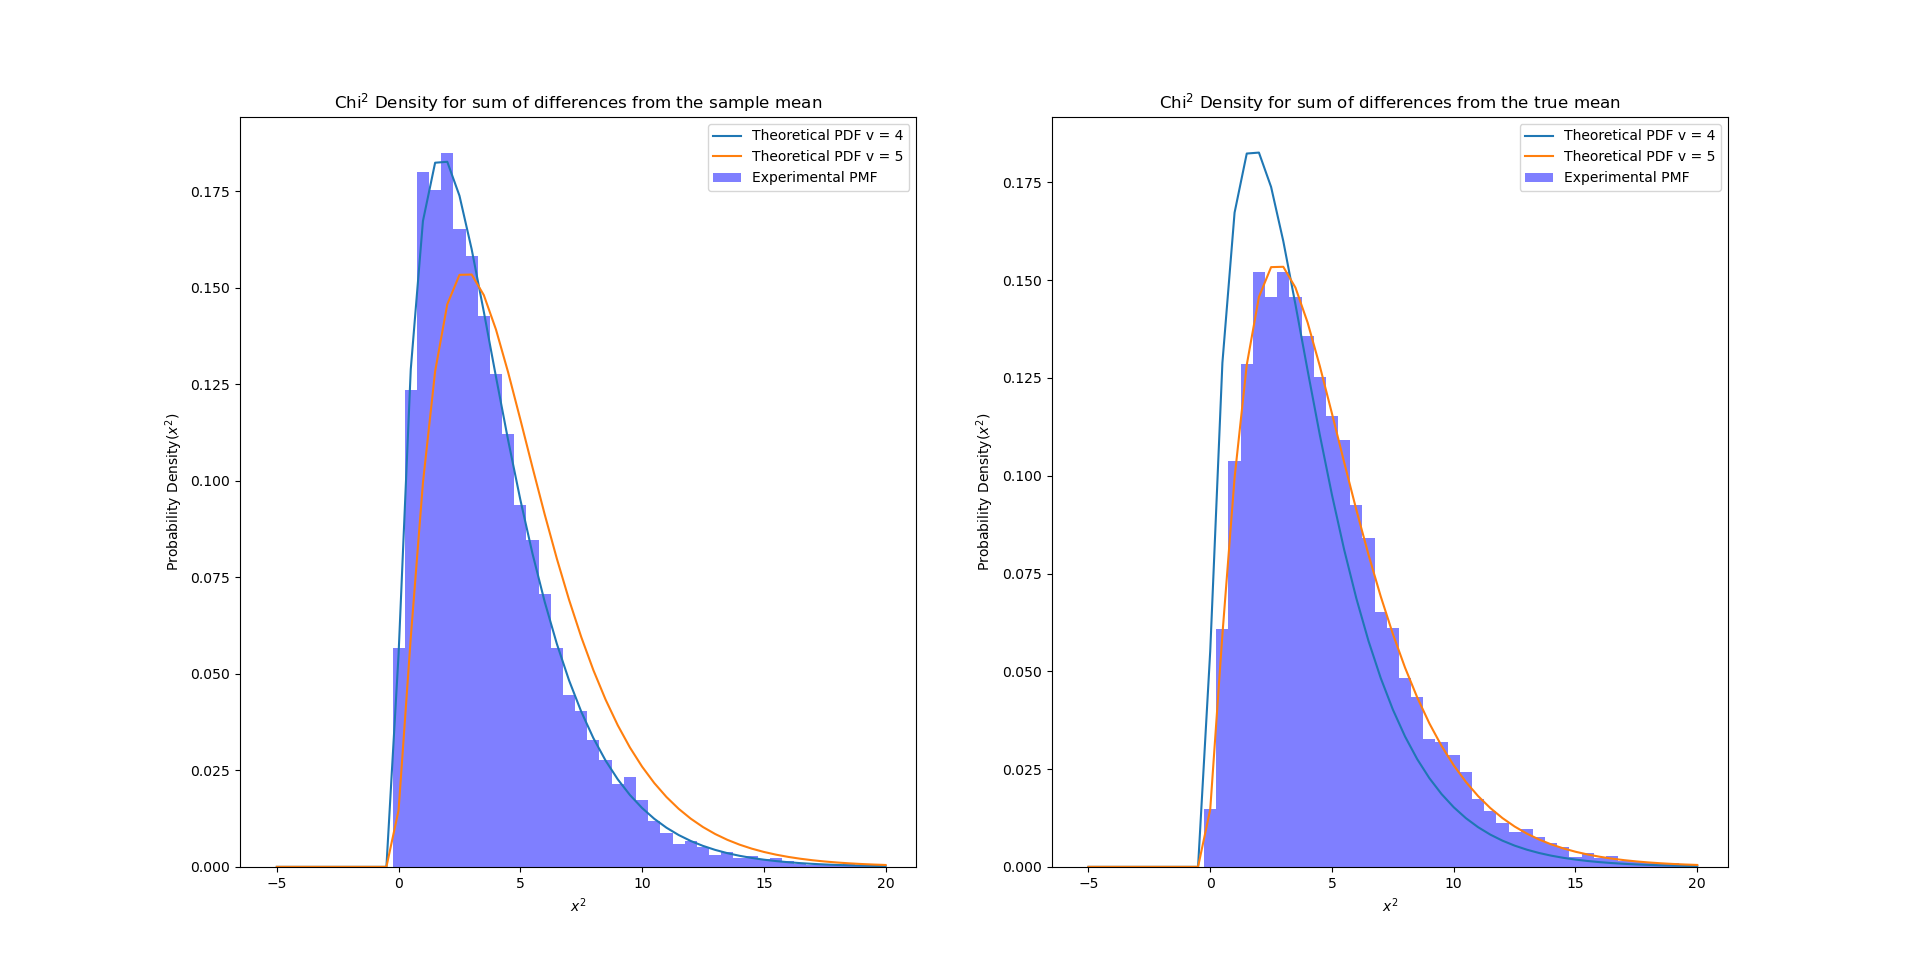
\includegraphics[width=0.95\textwidth]{chiSquared.png}
                \caption{PDFs and CDFs of the Chi$^2$ distribution with true mean of 2.5}
                \label{fig:chi2}
            \end{figure}
            The resulting plots for this experiment can be seen in \cref{fig:chi2}. On each plot the pdf for degrees of freedom 4 and 5 are plotted alongside the corresponding pdf. The left plot is a chi squard density from using the sample variance. From this plot we can see that it lines up very closely with the pdf where $\nu = 4$. The plot on the right is the density from using the difference between the true mean, and it can be seen that this lines up very closely with the pdf of $\nu = 5$. This indicates that the degrees of freedom of the sample pmf is influenced by how close you sample mean is to your true mean, with it being closer resulting in a higher $\nu$ value.
            \par
            From both plots, it can be concluded that a chi squared density can be applied to a normally distributed random variable as the experimental results line up with the theoretical ones.
    \section{Conclusion}
        From all plots in \cref{sec:normalExp} it can be seen that there is a significant amount of variation in the data compared to plots in \cref{sec:tExp,sec:chi2Exp}. This indicates that accuracy in statistical analysis can be improved by taking more measurements.
    % \Urlmuskip=0mu plus 1mu\relax
    \bibliography{bibliography}
    \bibliographystyle{IEEEtran}

    \begin{appendices}
        \section{Normal Distribution Code}
            \pythonexternal{NormalDensity.py}
        \section{t Distribution Code}
            \lstinputlisting{StudentT.m}
        \section{Chi Squared Density Code}
            \pythonexternal{ChiSquared.py}
            
    \end{appendices}
\end{document}